\section{APLIKASI PENDETEKSI BANJIR}

\subsection{KENAPA HARUS APLIKASI INI ?}
\begin{enumerate}
\item Membantu orang apabila terjad bencana banjir
\item Menanggulangi bencana banjir dan menyiapkan warga akanterjadna bencana
\end{enumerate}

\subsection{Alat dan Bahan} 
\begin{enumerate}
\item Arduino. Pada gambar \ref{labelgambar1} merupakan gambar arduino yang digunakan pada pembuatan alat ini
	\begin{figure}[htbp]
	\centering
	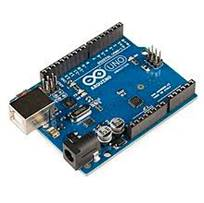
\includegraphics[width=0.5\textwidth]{figures/ALAT_PENDETEKSI_BANJIR/arduino1c}
	\caption{Arduino}
	\label{labelgambar1}
	\end{figure}

\item Bread board. Pada gambar \ref{labelgambar2} merupakan gambar Bread Board yang digunakan pada pembuatan alat ini.
	\begin{figure}[htbp]
	\centering
	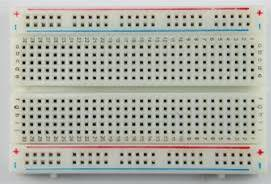
\includegraphics[width=0.5\textwidth]{figures/ALAT_PENDETEKSI_BANJIR/bread_board_1c}
	\caption{Bread Board}
	\label{labelgambar2}
	\end{figure}

\item Kabel jumper. Pada gambar \ref{labelgambar3} merupakan gambar Kabel Jumper yang digunakan pada pembuatan alat ini.
	\begin{figure}[htbp]
	\centering
	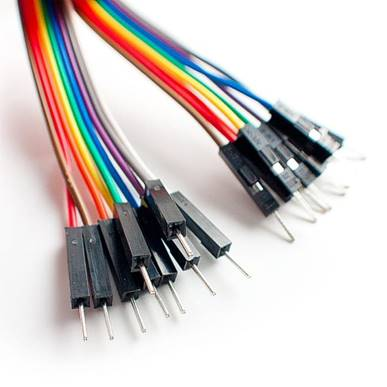
\includegraphics[width=0.5\textwidth]{figures/ALAT_PENDETEKSI_BANJIR/kabel_jumper_1c}
	\caption{Kabel Jumper}
	\label{labelgambar3}
	\end{figure}

\item Pendeteksi sensor ultrasonik. Pada gambar \ref{labelgambar4} merupakan gambar Pendeteksi Sensor Ultrasonik yang digunakan pada pembuatan alat ini.
	\begin{figure}[htbp]
	\centering
	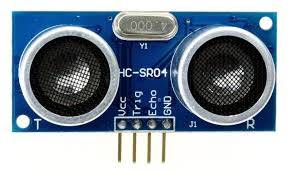
\includegraphics[width=0.5\textwidth]{figures/ALAT_PENDETEKSI_BANJIR/pendeteksi_sensor_ultrasonik_1c}
	\caption{Pendeteksi Sensor Ultrasonik}
	\label{labelgambar4}
	\end{figure}

\item Arduino IDE.  Pada gambar \ref{labelgambar5} merupakan gambar Arduino IDE yang digunakan pada pembuatan alat ini.
	\begin{figure}[htbp]
	\centering
	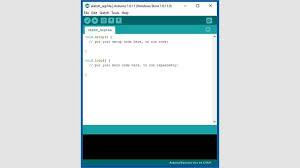
\includegraphics[width=0.5\textwidth]{figures/ALAT_PENDETEKSI_BANJIR/arduino_IDE_1c}
	\caption{Arduino IDE}
	\label{labelgambar5}
	\end{figure}

\item Lampu LED.  Pada gambar \ref{labelgambar6} merupakan gambar Arduino IDE yang digunakan pada pembuatan alat ini.
	\begin{figure}[htbp]
	\centering
	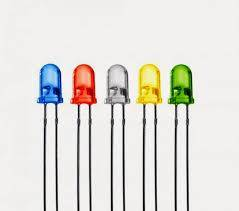
\includegraphics[width=0.5\textwidth]{figures/ALAT_PENDETEKSI_BANJIR/lampu_led_1c}
	\caption{Lampu LED}
	\label{labelgambar6}
	\end{figure}
\end{enumerate}

\subsection{CODE PROGRAMNYA}
\begin{lstlisting}
//defines pins numbers
const int trigPin = 10;
const int echoPin = 11;
//const int buzzer = 12;
const int ledPin= 13;

// defines variables
long duration;
int distance;
int safetyDistance;

void setup() {
  pinMode (trigPin, OUTPUT); // Sets the trigPin as an Output
  pinMode (echoPin, INPUT); // set the echoPin as an Input
 //pinMode(buzzer, OUTPUT);
 pinMode (ledPin, OUTPUT);
 Serial.begin(9600); // Starts the serial communication
}

void loop() {
  // Clears the trigPin
  digitalWrite(trigPin, LOW);
  delayMicroseconds(2);
  // Set the trigPin on HIGH state for 10 micro seconds
  digitalWrite(trigPin, HIGH);
  delayMicroseconds(5);
  digitalWrite(trigPin, LOW);
  // Reads the echoPin, returns the second wave travel time in microseconds
  duration = pulseIn(echoPin, HIGH);
  // Calculating the distance
  distance = duration*0.034/2;
  safetyDistance = distance;
  if (safetyDistance <=10){
    // digitalWrite(buzzer, HIGH);
    digitalWrite(ledPin, HIGH);
  }
  else{
    //digitaWrite (Buzzer, LOW);
    digitalWrite(ledPin, LOW);
  }
 // Prints the distance on the Serial Monitor
 Serial.print("Distance: ");
 Serial.println (distance);
}
\end{lstlisting}

\subsection{BAGAIMANA CARA PASANG NYA ?}
\begin{enumerate}
\item Masukan lampu led di port GND dan Port 13
\item Pasang Pendeteksi sensor HC-SR04
\item Sambungkan kabel juper nya dengan urutan port 11 dan 10 di masukan di port echo danport trig
\item Masukan port 5v ke port vcc
\item Masukan port GND ke Port GND
\end{enumerate}

\subsection{FOTO ALAT PENDETEKSI BANJIR}
Pada gambar \ref{labelgambar7} merupakan gambar alat pendeteksi banjir
\begin{figure}[htbp]
	\centering
	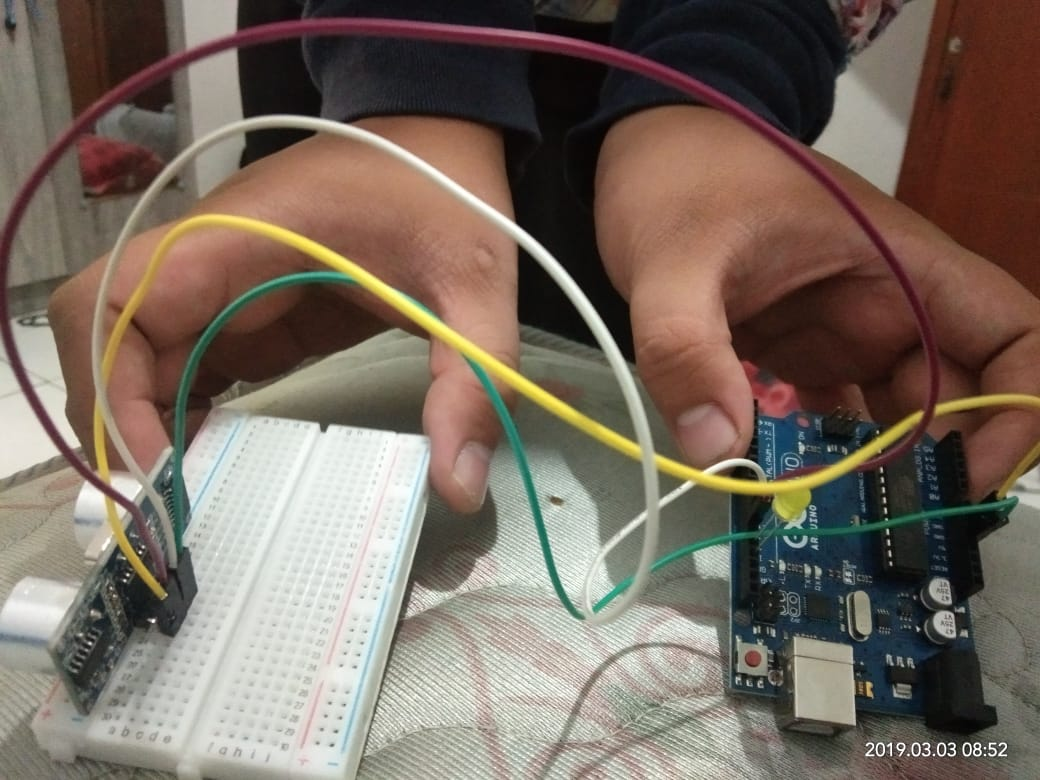
\includegraphics[width=0.5\textwidth]{figures/ALAT_PENDETEKSI_BANJIR/foto_alat_pendeteksi_banjir}
	\caption{Alat Pendeteksi Banjir}
	\label{labelgambar7}
	\end{figure}

\subsection{KESIMPULAN}
Banjir merupakan bencana yang tidak bisa di duga duga oleh manusia dan banjir bisa terjadi dimana mana. Karena itu aplikasi ini dibuat agar orang orang bisa bersiaga menghadapi bencana banjir
 